We shall now introduce the augmented complex zonotope set
representation and describe the over-approximation of its intersection
with a sub-parallelotope.  In Lemma~\ref{lem:motivation}, we have shown that the
intersection of a suitably aligned interval zonotope with a
sub-parallelotope can be computed exactly by a simple algebraic
formula.  Afterwards, in Lemma~\ref{lem:minsum-intersection}, we gave
an over-approximation and also an under-approximation of the intersection
between a sub-parallelotope and the Minkowski sum of a convex set with
interval zonotope.  Motivated by this, we specify an augmented complex zonotope
as a Minkowski sum of a template complex zonotope and an interval
zonotope.  The idea behind such a representation is that the interval
zonotope part is used to compute the intersection with a
sub-parallelotope, while the template complex zonotope may capture
positive invariance based on complex eigenstructure.
%
\begin{definition}
Let us consider a template complex zonotope
$\tcztope{\ptemp}{\cen}{\sfact}\subseteq\compnums^n$ and an interval
zonotope $\iztope{\stemp}{\lb}{\ub}\subseteq\reals^n$.  Then the
following is the representation of an augmented complex zonotope.
%
\[
\acztope{\ptemp}{\cen}{\sfact}{\stemp}{\lb}{\ub}=\minsum{\tcztope{\ptemp}{\cen}{\sfact}}{\iztope{\stemp}{\lb}{\ub}}.
\]
%
\end{definition}
%
Now we state an over-approximation by
an augmented complex zonotope for the
the intersection between an augmented complex zonotope and a
sub-parallelotope.  We also derive a bound on the over-approximation
error expressed in terms of the Hausdorff distance.

We recall the notation used in Lemma~\ref{lem:minsum-intersection}.
We define the Hausdorff distance as follows.
%
\[
\hausdorff{S_1}{S_2}=\max\lt(\max_{x\in S_1}\min_{y\in
S_2}\norm{x-y},\max_{x\in S_2}\min_{y\in S_1}\norm{x-y}\rt).
\]
%
\begin{theorem}~\label{thm:main-intersection}
Let us denote
$\Psi_1=\acztope{\ptemp}{\cen}{\sfact}{\pinv{\qtemp}}{\lb}{\ub}\bigcap\ptope{\qtemp}{\plb}{\pub}$,\\
$\Psi_2=\ptope{\qtemp}{\plb}{\pub}$ and
$\Psi_3=\acztope{\ptemp}{\cen}{\sfact}{\pinv{\qtemp}}{\join{\lb}{\plb}}{\meet{\ub}{\pub}}$.
Let us consider that
%
\begin{align*}
& \lb\leq\join{\lb}{\plb}\leq\meet{\ub}{\pub}\leq\ub~\text{and}~\forall
 i\in \set{1,...,k}\\
& ~\tcztope{\compid{i}\qtemp\ptemp}{\compid{i}\qtemp\cen}{\sfact}\order\tcztope{\qtemp\ptemp}{\qtemp\cen}{\sfact}.~\numberthis\label{eqn:acz-intersection2}\\
\text{Then}~~&\Psi_1\bigcap\Psi_2\subseteq\Psi_3~\text{and}~\numberthis\label{eqn:acz-intersection3}\\
& \hausdorff{\Psi_1\bigcap\Psi_2}{\Psi_3}\leq\norm{\mymatrix{\pinv{\qtemp}
 & \pinv{Y}}}\hausdorff{\tcztope{\qtemp\ptemp}{\qtemp\cen}{\sfact}}{0}.~\numberthis\label{eqn:acz-intersection4}
\end{align*}
%
\end{theorem}
%
\begin{proof}
Let us denote $S=\tcztope{\ptemp}{\cen}{\sfact}$.  We get by
Equation~\ref{eqn:acz-intersection2} and
Theorem~\ref{thm:suff-inclusion} that $
\forall i\in\set{1,...,k},~\compid{i}\qtemp S\subseteq \qtemp S.$

Then by Lemma~\ref{lem:minsum-intersection}, we get
%
\begin{align*}
& \text{Then}~~\mymatrix{0\\ Y^T}S \oplus\mymatrix{\qtemp\\
 Y^T}\iztope{\pinv{\qtemp}}{\join{\lb}{\plb}}{\meet{\ub}{\pub}}
 \\ & \subseteq\mymatrix{\qtemp\\
 Y^T}\lt(\lt(S\oplus \iztope{\pinv{\qtemp}}{\lb}{\ub}\rt)\bigcap\ptope{\qtemp}{\plb}{\pub}\rt)~\numberthis\label{proof-acz-intersection1}\\
 &\subseteq \mymatrix{\qtemp\\
 Y^T}\lt(S \oplus\iztope{\pinv{\qtemp}}{\join{\lb}{\plb}}{\meet{\ub}{\pub}}\rt).\numberthis~\label{proof-acz-intersection2}
\end{align*}
%
By the definition of an augmented complex zonotope, we have
%
\[
\Psi_1=S\oplus\iztope{\pinv{\qtemp}}{\lb}{\ub},~~
\Psi_3=S \oplus\iztope{\pinv{\qtemp}}{\join{\lb}{\plb}}{\meet{\ub}{\pub}}.
\]
%
Then by Equation~\ref{proof-acz-intersection2} we get
%
\[
\mymatrix{\qtemp\\ Y^T}\lt(\Psi_1\bigcap\Psi_2\rt)\subseteq\mymatrix{\qtemp\\ Y^T}\Psi_3.
\]
%
As $\mymatrix{\qtemp\\ Y^T}$ is a non-singular (invertible) matrix, we get
Equation~\ref{eqn:acz-intersection3}.

Next, we shall prove Equation~\ref{eqn:acz-intersection4}.
%
By Equation~\ref{proof-acz-intersection1}
and~\ref{proof-acz-intersection2} we get
%
\begin{align*}
& \hausdorff{\mymatrix{\qtemp\\
Y^T}\lt(\Psi_1\bigcap\Psi_2\rt)}{\mymatrix{\qtemp\\ Y^T}\lt(\Psi_3\rt)}
\leq\hausdorff{\qtemp S}{0}.\\
&\implies \hausdorff{\Psi_1\bigcap\Psi_2}{\Psi_3}\\
& \leq\norm{\mymatrix{\pinv{\qtemp}
& \pinv{Y}}}\hausdorff{\mymatrix{\qtemp\\
Y^T}\lt(\Psi_1\bigcap\Psi_2\rt)}{\mymatrix{\qtemp\\ Y^T}\lt(\Psi_3\rt)}\\
& \leq \norm{\mymatrix{\pinv{\qtemp} &
 \pinv{Y}}}\hausdorff{\qtemp S}{0}=\norm{\mymatrix{\pinv{\qtemp}
 & \pinv{Y}}}\hausdorff{\tcztope{\qtemp\ptemp}{\qtemp\cen}{\sfact}}{0}.~\hspace{2em}\qedhere
\end{align*}
%
\end{proof}
%
In Theorem~\ref{thm:main-intersection}, the above bound on the over-approximation error is positively
correlated with
$\qtemp\ptemp$ and $\qtemp\cen$, i.e., the orientation between the
sub-parallelotopic template $\qtemp$ the the primary template $\ptemp$
and primary offset $\cen$.  The bound is zero when the $\qtemp$ is orthogonal to
$\ptemp$ and $\cen$, in which case the we can exactly specify the
intersection by the augmented complex zonotope.
%
\begin{example}
Let us consider an augmented complex zonotope\\
${S_1=\acztope{V}{0}{\repmat{1}{3}{1}}{\pinv{K}}{1}{1}}$ and a
sub-parallelotope $S_2=\ptope{K}{0.5}{0.5}$ where
%
\[
V = \mymatrix{
1+2\iota & 1 & 0\\
1-\iota & 0 & 0\\
0 & 0 & e
},~~
K = \mymatrix{0 & 0 & 1}.
\]
%
for some $e\in \reals$.  Then
%
\[
S_1\bigcap S_2\subseteq \acztope{V}{0}{\repmat{1}{3}{1}}{K}{0.5}{0.5}.
\]
%
Furthermore, the over-approximation error is proportional to
$\absolute{e}$, which is equal to $\norm{KV}$.  For example, when
$e=0$, then the over-approximation error is zero, i.e., the above is
an equality.  On the other hand, when $e\neq 0$, then the Hausdorff
distance between the intersected set and the over-approximation is
equal to $e$.  This is illustrated in
Figures~\ref{fig:overapp1},~\ref{fig:overapp1} and ~\ref{fig:overapp1}
that display the projection of the intersected set and the
over-approximation along the $XY$ and $YZ$ planes for ${e=0}$, $e=0.5$
and $e=1$, respectively.
\end{example}
%
%
\begin{figure}
\center
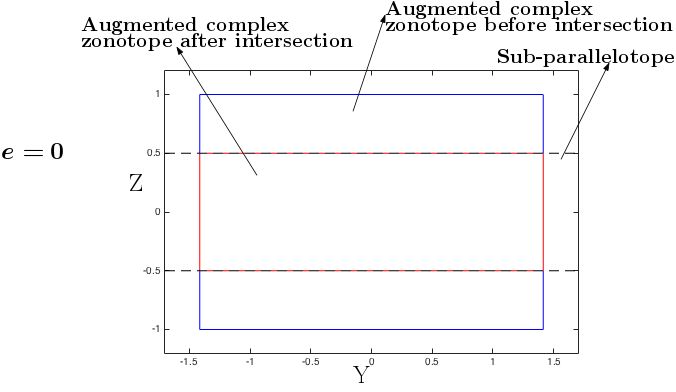
\includegraphics[scale=0.5]{fig/CZtopes/intersectionyz1.png}
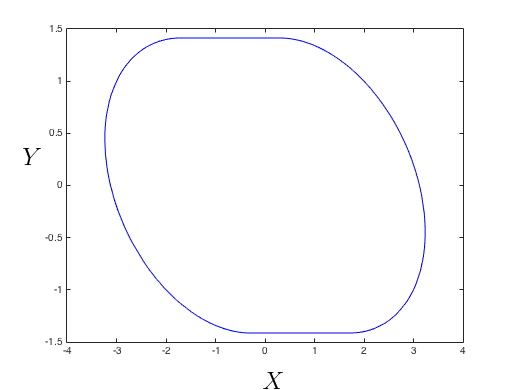
\includegraphics[scale=0.5]{fig/CZtopes/intersectionxy.png}
\caption{Over-approximation of intersection for $e=0$.}~\label{fig:overapp1}
\end{figure}
%
%
\begin{figure}
\center
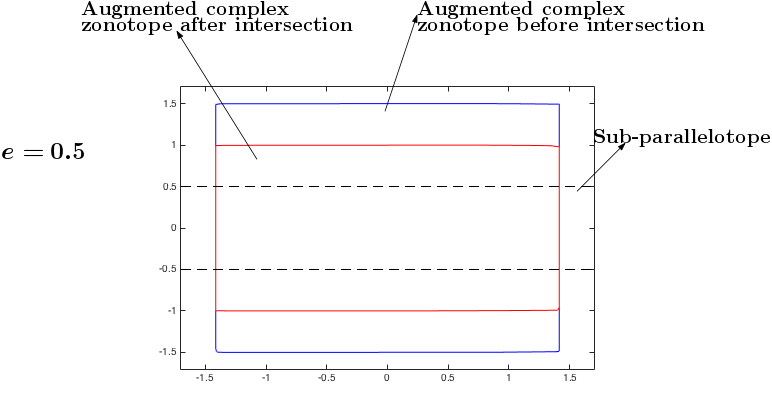
\includegraphics[scale=0.5]{fig/CZtopes/intersectionyz2.png}
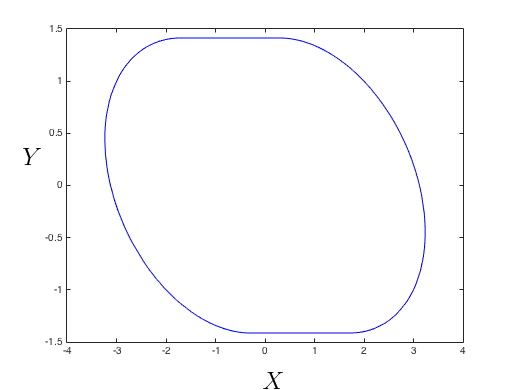
\includegraphics[scale=0.5]{fig/CZtopes/intersectionxy.png}
\caption{Over-approximation of intersection for $e=0.5$.}~\label{fig:overapp2}
\end{figure}
%
\begin{figure}
\center
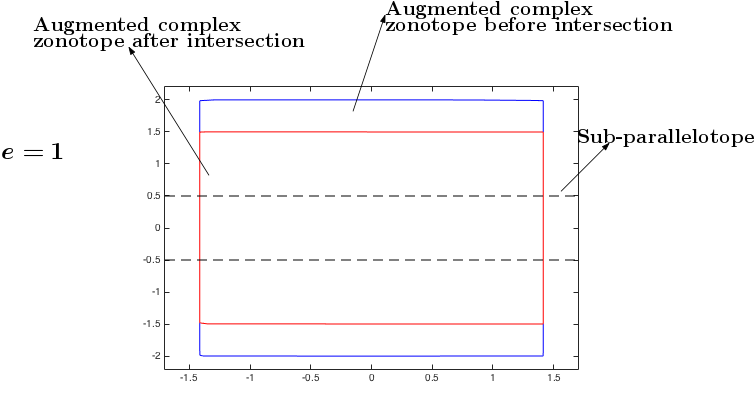
\includegraphics[scale=0.5]{fig/CZtopes/intersectionyz3.png}
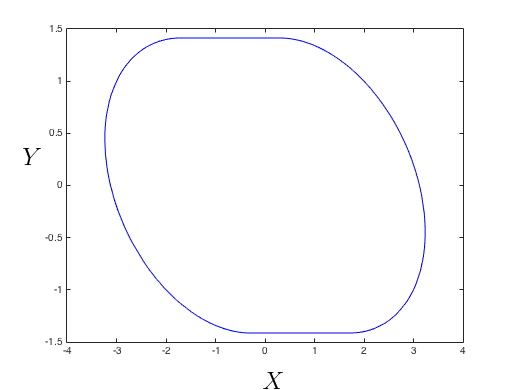
\includegraphics[scale=0.5]{fig/CZtopes/intersectionxy.png}
\caption{Over-approximation of intersection for $e=1$.}~\label{fig:overapp3}
\end{figure}
%
